\documentclass[_ArquivoPrincipal.tex]{subfiles}

\begin{document}

%==================================================================================================
\chapter{Fundamentação Teórica} \label{FT}
%==================================================================================================

Exemplo de equação:


\begin{equation}
    \begin{centering}
    \int_\Gamma{\sigma^T\cdot \mathbf{n}d\Gamma}+\int_\Omega{\nabla \sigma d\Omega}=\mathbf{f}
    \text{,}
    \end{centering}
    \label{eq:EqGlobEu}
\end{equation}

Essa foi a Eq. \eqref{eq:EqGlobEu}

Referência textual a \citeonline{tezduyar1991stabilized} é quando está no meio da sentença. Parcial é quando está ao final \cite{tezduyar1991stabilized}.

Exemplo de figura pode ser visto na figura \ref{fig:BalMas}

\begin{figure}[h]
    \centering
    \caption{Taxa de fluxo de massa em um elemento infinitesimal permeável.}
    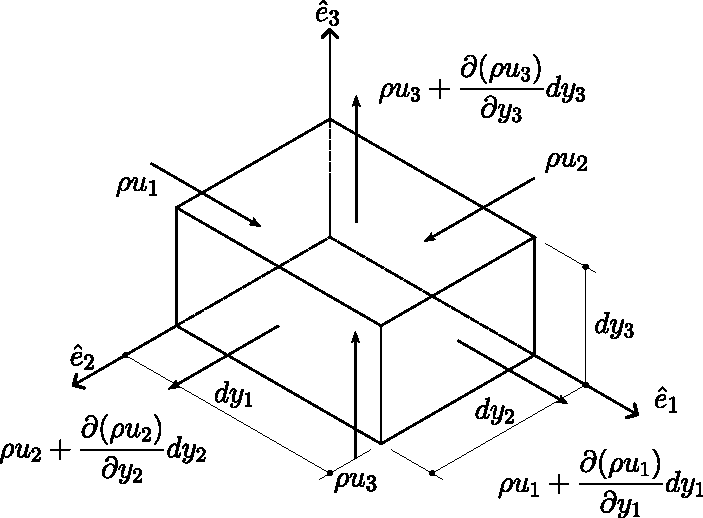
\includegraphics[width=.5\linewidth]{Figuras/BalMas.pdf}
    \\Fonte: Autoria Própria (\the\year).
    \label{fig:BalMas}
\end{figure}

\end{document}